\documentclass[12pt]{article}
\usepackage{natbib}
\usepackage{hyperref}
\usepackage{graphicx}
\usepackage{caption}
\usepackage{subcaption}
\usepackage[margin=0.75in]{geometry}
\usepackage{flafter}
\usepackage{setspace}
\usepackage{titlesec}
\usepackage{adjustbox}
\usepackage{floatrow}
\usepackage{rotating}


\setcounter{tocdepth}{6}
\setcounter{secnumdepth}{6}



%%%%%%%%% set up outlining stuff
\usepackage{outlines}
\usepackage{enumitem}
\setenumerate[1]{label=\Roman*.}
\setenumerate[2]{label=\Alph*.}
\setenumerate[3]{label=\roman*.}
\setenumerate[4]{label=\alph*.}
\setenumerate[5]{label=\roman*.}
%%%%%%%%%

\graphicspath{{./Figures/}}


\title{Using Git and GitHub -- Maddie's top commands}
\author{MMH}


\begin{document}
\maketitle
  
%%%%%%%%%%%%%%%%%%%%%%%%%%%%%%%%%%%%%%%%%%%%%%%%%%%%%
\section*{Introduction}

git = local\\
GitHub = git with friends\\
Git repositories should be thought of as ``projects"\\

This compilation of git commands isn't comprehensive, but it covers the commands that I use on a regular basis. I should preface all of this by mentioning that {\it I use the command line}, but you don't have to. If you prefer GUI work, you can download the GitHub GUI at \href{url}{https://desktop.github.com/}. It's useful for both git and GitHub. And I know next to nothing about how to use it.\\ \\

Some other AMAZING resources for the MOD group:\\
\href{url}{https://github.com/modscripps} \\ 
\href{url}{https://github.com/OceanMixingGroup}\\
Guys, we can't let Jonathan Nash be way better at version control than we are...

\begin{figure}[hbt]
	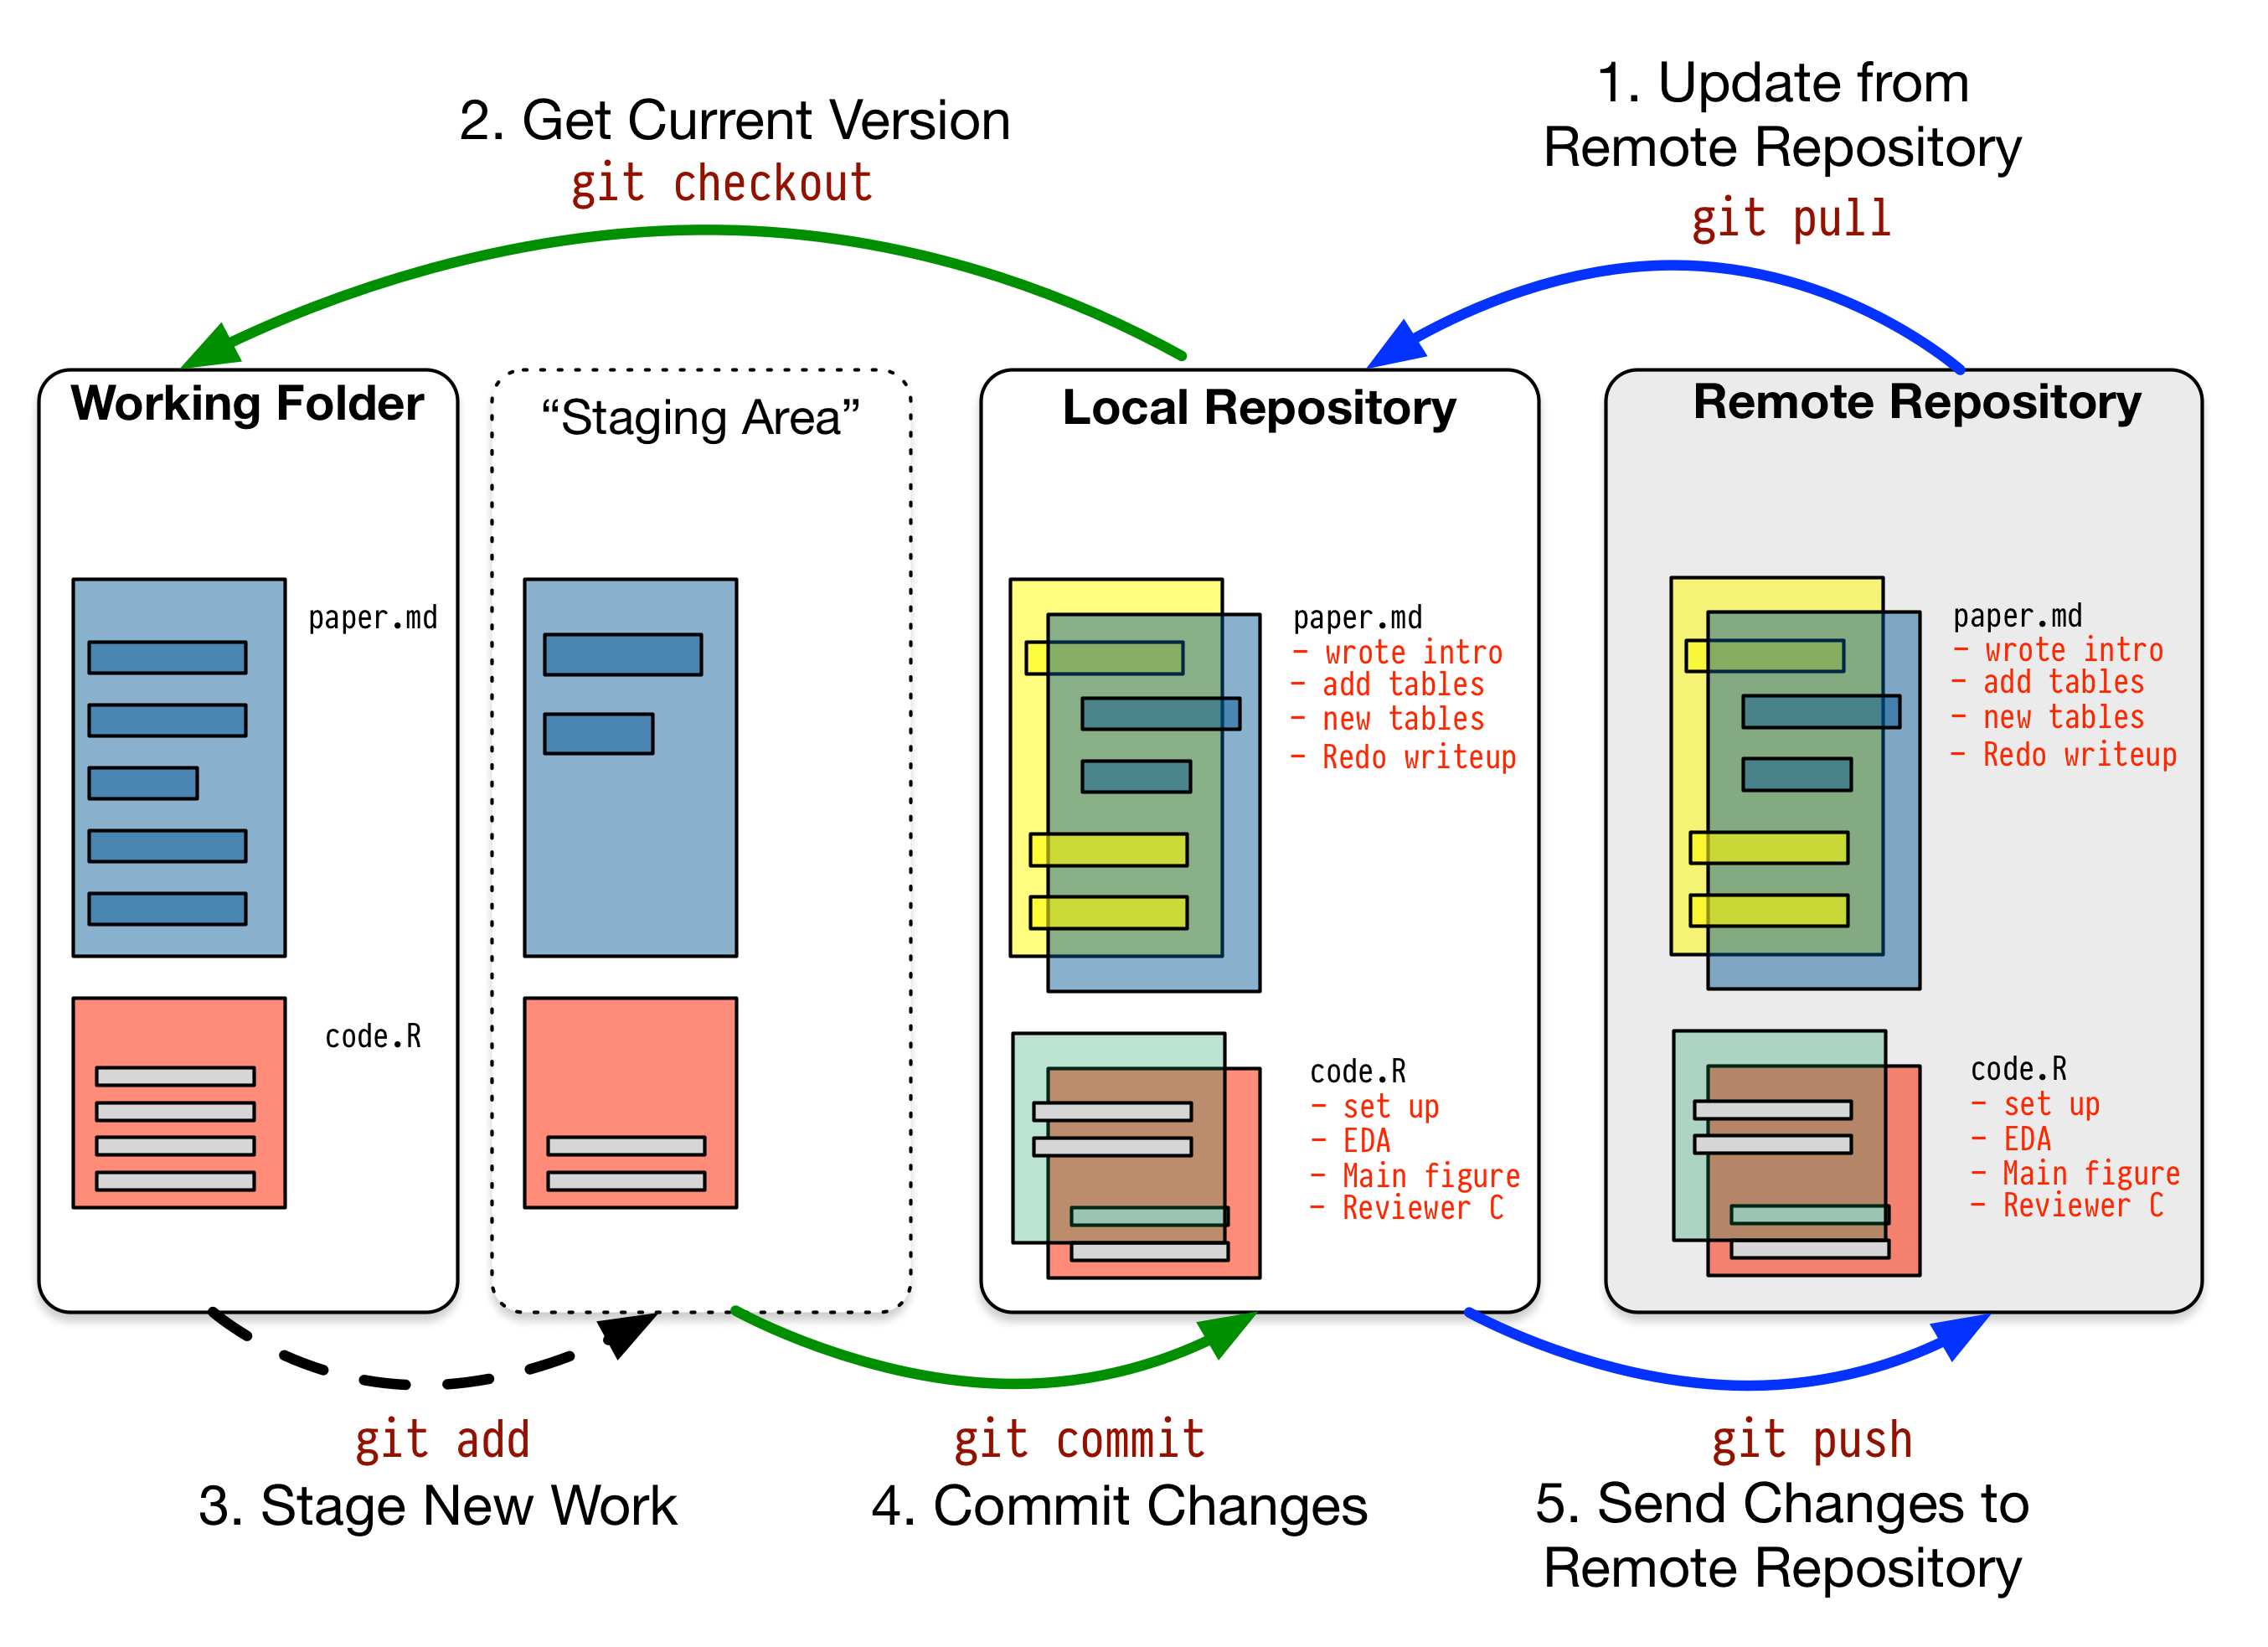
\includegraphics[width=\textwidth]{git-basic.png}
	\caption{Okay, so this is a nice figure to contextualize what's going on with git.}
\end{figure}



%%%%%%%%%%%%%%%%%%%%%%%%%%%%%%%%%%%%%%%%%%%%%%%%%%%%%
\clearpage
\section*{Local {\bf git} commands}

\begin{outline}[enumerate]
  \1 Making Changes  	
        \2 {\bf git init} 
       	 	\3 creates a git repository 
            		\\ {\it mkdir yourdirectoryname }
            		\\ {\it cd yourdirectoryname}
            		\\ {\it vi README.md}
		         \\ {\it git init}
                			\4 ``.md" stands for markdown
                			\4 This is for best practices purposes
        \2 {\bf git add}
        		\3 adds files within your working directory into the staging area
        		\\ {\it git add -A}
        			\4 adds ALL files
            	\3 if the repository contains a file called .gitignore, files with designated file extensions or within specified subdirectories will not be added
        		\\ {\it vi .gitignore}
        		\\ {\it git add .gitignore}
        			\4 Examples of .gitignore files can be found at \href{url}{https://github.com/github/gitignore}
        			\4 It has to be added to the repo in order to work!!
        \2 {\bf git commit}
            	\3 takes what is in staging directory and puts into git working directory
        		\\ {\it git commit -m ``YOUR MESSAGE HERE"}
        			\4 commits changes in staging area
        			\4 `-m' adds a message so that you can comment on your changes
\1 Visualizing Progress			
	\2 {\bf git status}
        		\3 shows the status of your woking directory and staging area relative to the current git repo
        \2 {\bf git diff}
        		\3 sees all content and understands in terms of additions and removals
            	\3 more complicated than git status; gives more detail on the file changes specified in git status
 \1 Making BIG changes -- Using Branches    
             	\\ for more info see: \href{url}{https://www.atlassian.com/git/tutorials/using-branches}   
        \2 {\bf git branch}
        		\3 creates a new line of development
        		\3 Use this when you are about to make major changes, or changes that might break things
        		\\ {\it git branch $<$branch-name$>$}
        			\4 git branches must have one word names
        			\4  main branch is always called ``master"
	\2 {\bf git checkout}
            	\3 use to begin operating in a project branch
                		\\ {\it git checkout $<$branch-name$>$}
            			\4 must move into the branch before committing devilish changes!
    	\2 {\bf git merge}
        		\3 merges changes from a branch into the directory you are currently working in
        		\3 to merge your $<$branch-name$>$ changes back into the main branch:
        			\\ {\it git checkout master}
    			\\ {\it git merge $<$branch-name$>$}            

\1 Fixing things
             	\\ for more info see: \href{url}{https://www.atlassian.com/git/tutorials/undoing-changes}   
	\2 {\bf git log}
		\3 Displays the commit history 
		\3 lists codes or ``commits" 
	\2 {\bf git checkout}
		\3 use to check out an old version of the file
			\\ {\it git checkout $<$head$>$ $<$filename$>$}
	\2 {\bf git reset}
		\3 Undo local changes
			\\ {\it git reset}
				\4 Resets the staging area to match the most recent commit, but leaves the working directory unchanged
			\\ {\it git reset --hard}
				\4 Resets staging area AND working directory
					

\end{outline}

%%%%%%%%%%%%%%%%%%%%%%%%%%%%%%%%%%%%%%%%%%%%%%%%%%%%%
\clearpage
\section*{{\bf GitHub} commands}
             	For more info see: \href{url}{https://www.atlassian.com/git/tutorials/syncing}   
\begin{outline}[enumerate]
\1 Set up remote
	\2 {\bf git remote}
		\3 list and add connections to remote repositories (like GitHub repos!)
			\\ {\it git remote add  $<$name$>$ $<$remote-url$>$}
    				\4 assign a remote repository to  a git workspace on your local machine
				\4 $<$name$>$ is most often ``origin"
				\4 now, any $<$remote-url$>$ that follows can be replaced with the chosen $<$name$>$
	\2 {\bf git clone}
    		\3 make a copy of someone else's repository to your own computer
    			\\ {\it git clone $<$remote-url$>$}
	\2 {\bf git fork}
    		\3 different from cloning--this continuously tracks with the master;
    		\3 use this if you plan to make a contribution back to the master with a useful change
\1 Interact with remote
       	\2 {\bf git push}
    		\3 pushes changes up to a remote repository
    			\\ {\it git push $<$remote-url$>$ master}
	\2 {\bf git pull}
		\3 pull changes from a remote repository into the current repo
			\\ {\it git pull  $<$remote-url$>$}
		\3 If you are the owner of a shared repository on github, you will use this command to pull changes made by other users into the master branch
\1 Fix things
	\2 {\bf git revert}
		\3 Undoes, but still tracks!, an entire commit
		\3 Because it still tracks, it is safer to use in a shared repository than {\it git reset}
			\\ {\it git revert}
			\\ OR {\it git revert $<$commit$>$}
	\2 {\bf git rebase}
		\3 use when a development branch gets way ahead of the master to reflect the development changes instead of the master history with user changes overlaid
\end{outline}
\end{document}

%Gists are for code snippets you want to share, but don?t need a whole repo